\documentclass[a4paper,12pt]{article}
\usepackage[T1]{fontenc}
\usepackage[margin=0.5in]{geometry}
\usepackage{graphicx}
\graphicspath{ {./images/} }
\usepackage{amsmath}
\usepackage{listings}
\usepackage{xcolor}
\usepackage{subfig}
\usepackage{hyperref}
\newcommand{\Mod}[1]{\ (\mathrm{mod}\ #1)}



\definecolor{codegreen}{rgb}{0,0.6,0}
\definecolor{codegray}{rgb}{0.5,0.5,0.5}
\definecolor{codepurple}{rgb}{0.58,0,0.82}
\definecolor{backcolour}{rgb}{0.95,0.95,0.92}

\lstdefinestyle{mystyle}{
    commentstyle=\color{codegreen},
    keywordstyle=\color{magenta},
    numberstyle=\tiny\color{codegray},
    stringstyle=\color{codepurple},
    basicstyle=\ttfamily\footnotesize
}
\lstset{style=mystyle}

\begin{document}

\title{ElGamal Encryption System - Documentation }
\author{Krzysztof Piotrowski and Jakub Tomkiewicz}
\date{11th of January 2022}
\maketitle

\section{Description of the used algorithm}

ElGamal is a public-key cryptosystem created in 1985 by Taher ElGamal that uses an asymmetric key encryption algorithm. 
Cryptosystem uses a protected exchange method through a public network called Diffie-Hellman key exchange.

Cipher is based on solving discrete logarithms in a large prime. 
The advantage of the cryptosystem is that the same encrypted plaintext is, each time, a different ciphertext.
However, as a disadvantage, the ciphertext is much longer than plaintext.

\section{Functional description of the application}

ElGamal cryptosystem application consist of key generation, encryption operation and decryption operation.
In order to generate public and private keys Alice needs to:
\begin{enumerate}
\item   Choose a prime \textbf{\textit{p}} and a generator \textbf{\textit{g}} from cyclic group \textbf{\textit{$ Z\otimes p $}}
\item   Choose a random $x \in (2,q-1)$ (where \textbf{\textit{q}} is order of cyclic group \textbf{\textit{$ Z\otimes p $}} )
\item	Compute $ h = g^x \Mod p $
\item	Publish \textbf{\textit{p}}, \textbf{\textit{q}}, \textbf{\textit{g}} and \textbf{\textit{h}} as \textbf{public key}
\item   Publish \textbf{\textit{x}} as \textbf{private key}
\end{enumerate}
Bob encrypts message m using public key from Alice:
\begin{enumerate}
\item	Chose random $ y \in (2,q-1) $
\item	Compute shared secret $ s = h^y \Mod p$
\item	Compute $ c_1 = g^y \Mod p $
\item	Encrypt m using formula $ c_2 = m \times s \Mod p $
\item	Publish ($c_1, c_2$) to Alice
\end{enumerate}
Alice having cipertext ($c_1, c_2$) from Bob and public key to decrypt message needs to:
\begin{enumerate}
\item	Compute invert of shared secret $ s = c_1^{-x} \Mod p $
\item	Decrypt message  $ M = c_2 \times s \Mod p $
\end{enumerate}

\section{Description of designed code structure}
\subsection{Generating large prime number}
In order to generate a prime number, function \textbf{\textit{choosePrime}} is called. A loop iterates until proper prime numer is found and returned. 
During that process, first we reject all even numbers and then make two probabilistic tests for validity of prime number. Each test consists of 100 trials.
\begin{lstlisting}[language=Python]
  def choosePrime(nrOfBits):
    # true until find prime number
    while True:
        primeCandidate = getrandbits(nrOfBits)
        # check if even number
        if primeCandidate % 2 == 0:
            continue
        # make 100 fermat tests 
        if not fermatPrimalityTest(primeCandidate, 100):
            continue
        # make 100 miller-rabin tests
        if not millerRabinTest(primeCandidate, 100):
            continue
        return primeCandidate
\end{lstlisting}
Miller-Rabin primality test is a probabilic method that checks if given number is a prime.
\begin{lstlisting}[language=Python]
    def millerRabinTest(nr, nrOfTimes):
        r = 0 
        s = nr - 1

        # Look for r (r > 0) until the
        # following equation is true: nr = 2^d * r + 1
        while s % 2 == 0:
            r += 1
            s //= 2

        # iterate nrOfTimes times
        for i in range(nrOfTimes):
            # x = a^s % nr
            x = pow(randrange(2, nr - 1), s, nr)

            # continue if x is 1 or nr - 1
            if x == 1 or x == nr - 1:
                continue

            # iterate r - 1 times
            for i in range(r - 1):
                # x = x * x % nr
                x = pow(x, 2, nr)

                # break if x reach nr - 1
                if x == nr - 1:
                    break
            else:
                return False
        return True
\end{lstlisting}
\newpage
Fermat primality test is, like Miller-Rabin, probabilistic method to check whether given numer is a prime. It is based on the Fermat's Little Theorem that says: for every a (1 < a < n-1) $ a^{n-1} \Mod n = 1 $
\begin{lstlisting}[language=Python]
    def fermatPrimalityTest(nr, nrOfTimes):
        # iterate nrOfTimes times
        for i in range(nrOfTimes):
            # Fermat's little theorem says that for every a (that 1 < a < nr-1)
            # flowing equation is true: a^(nr-1) % nr = 1
            if pow(randint(2, nr - 2), nr - 1, nr) != 1:
                return False
        return True
\end{lstlisting}

\subsection{Key generation \& Encryption \& Decryption}
After we find proper prime number, we use it for cyclic group description that base on prime value. 
The order of prime cyclic group is always one less than prime value. Additionally, we need to find generator of that cyclic group. 
\begin{lstlisting}[language=Python]
    def cyclicGroupDescription(p):
        # Order of prime cyclic group is p - 1 as it has p - 1 elements in group
        q = p - 1
        # Get generator which is primitive root of prime number
        g = findPrimitiveRoot(p)
        return (p, q, g)
\end{lstlisting}
Due to the size of prime value we cannot search for all generators of cyclic group. 
Instead we will find primitive root \textbf{\textit{r}} for prime \textbf{\textit{p}} which values of $r^x \Mod p$ where \textbf{\textit{x}}  $\in [0, p-2]$ are different (thus fullfills generator requirements). 
\begin{lstlisting}[language=Python]
    def findPrimitiveRoot(p):
        if p == 2:
            return 1
        #the prime divisors of p-1 are 2 and (p-1)/2 
        #because p = 2x + 1 where x is a prime
        p1 = 2
        p2 = (p - 1) // p1
        #test random g's until one is found that is a primitive root mod p
        while True:
            g = randint(2, p - 1)
            #g is a primitive root if for all prime factors of p-1, p[i]
            #g^((p-1)/p[i]) (mod p) is not congruent to 1
            if not (pow(g, (p - 1) // p1, p) == 1):
                if not (pow(g, (p - 1) // p2, p) == 1):
                    return g
\end{lstlisting}
After getting whole cyclic group description we can start with generating keys for ElGamal. 
First we choose random value \textbf{\textit{x}} which will be treated as private key. 
After that we calculate \textbf{\textit{h}} value which will be used for encryption. 
Calulcated \textbf{\textit{h}} with \textbf{\textit{p}}, \textbf{\textit{q}} and \textbf{\textit{g}} will be treated as public key. 
\begin{lstlisting}[language=Python]
    def generateKeys(p, q, g):
        # choose random integer which will be treated 
        #as private key and used for h calculation 
        x = randint(2, q - 1) 
        # calculate h equal g^x mod p, will be used for encryption
        h = pow(g, x, p) 
        publicKey = (p, q, g, h)
        privateKey = x
        return (publicKey, privateKey)
\end{lstlisting} \newpage 
As mentioned above, encryption uses public key. 
We generate \textbf{\textit{y}} which is responsible for encryption calculations. 
With its usage we calculated shared secret. 
Encrypted message is kept in two pieces, in our code there are called \textbf{\textit{$c_1$}} and \textbf{\textit{$c_2$}}.
We stored them as so-called pairs for future decryption.
\begin{lstlisting}[language=Python]
    def encryption(messageBlocks, publicKey):
        p = publicKey[0] # Group (prime number)
        q = publicKey[1] # order
        g = publicKey[2] # generator
        h = publicKey[3] 
        encryptedBlocks = []
        for block in messageBlocks:
            encryptedPairs = []
            # randomly selected y for future calculations
            y = randint(2, q - 1)
            # compute shared secret
            s = pow(h, y, p)
            # first part of cipher text
            c1 = pow(g, y, p)
            for sign in block:
                #second part of cipher text
                c2 = (sign * s ) % p
                # keep both parts as a pair for decryption 
                encryptedPairs.append([c1,c2])
            #separate each block pairs 
            encryptedBlocks.append(encryptedPairs)
        return encryptedBlocks
\end{lstlisting}
Decryption takes private key and previously stored cipher pairs. We decrypt each block separately.
As in encryption, shared secret is computed with the use of private key and $c_1$. Its inverse with $c_2$ decrypt the message.
\begin{lstlisting}[language=Python]
    def decryption(encryptedBlocks, privateKey, group):
        messageBlocks = []
        for encryptedBlock in encryptedBlocks:
            block = []
            for pair in encryptedBlock:
                # compute inverse of shared secret as c1^(-x) mod p 
                s = pow(pair[0], -1 * privateKey, group)
                # decrypt message: c^2 * s mod p 
                m = (pair[1]* s) % group
                # add message to block
                block.append(m)
            # when whole block is decrypted, add to the rest of message blocks    
            messageBlocks.append(block)
        return messageBlocks
\end{lstlisting}
\subsection{Operations on blocks}

When we read text from the plaintext.txt, characters are being parsed to ASCII code and separated into 16 element blocks.
\begin{lstlisting}[language=Python]
    def convertMsgToBlocks(msg):
        blocks = []
        for char in msg:
            # convert char to nr
            blocks.append(ord(char))
        messageBlocks = [blocks[i:i+16] for i in range (0, len(blocks), 16)]
        return messageBlocks  
\end{lstlisting}
\newpage
After the decryption, blocks of numbers are parsed to strings and joined together.
\begin{lstlisting}[language=Python]
    def convertBlocksToMsg(messageBlocks):
        # placeholder for msg block
        oneMessageBlock = []

        # placeholder for msg
        msg = ''

        for block in messageBlocks:
            oneMessageBlock += block

        for element in oneMessageBlock:
            # convert nr to char
            msg += chr(element)
        return msg 
\end{lstlisting}
When a message was encrypted, function writes the encrypted blocks content as string into the ciphertext.txt file.
\begin{lstlisting}[language=Python]
    def writeEncryptedMessage(encryptedBlocks):
        # open ciphertext with write flag
        f = open("ciphertext.txt", "w")

        for block in encryptedBlocks:
            for element in block:
                f.write(str(element[0]) + ' ' + str(element[1]) + ' ')
        f.close
\end{lstlisting}
\section{Tests}

Our program was tested in comparison with website \href{https://www.debjitbiswas.com/elgamal/}{https://www.debjitbiswas.com/elgamal/} that offers online ElGamal encryption.
We will use small prime values as the above website cannot process 1024 bit numbers.

Input plaintext is being imported from the file plaintext.txt, and after being encrypted and decrypted, it is saved in file decryptedtext.txt
\subsection{Test for small prime}
\begin{figure}[h]%
    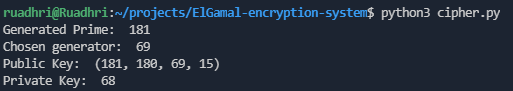
\includegraphics{smallPrime.PNG}%
    \centering 
    \caption{Values generated by the script}%  
\end{figure}%
  
\begin{figure}[h]%
    \centering
    \subfloat{{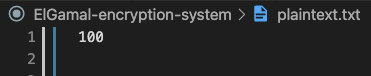
\includegraphics[width=6.5cm]{plaintextForSmallPrime.png} }}%
    \qquad
    \subfloat{{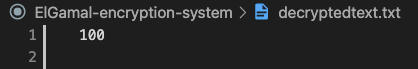
\includegraphics[width=8cm]{decryptedForSmallPrime.png} }}%
    \caption{Plain text vs decrypted text}%
\end{figure}
 
\begin{figure}[h]%
    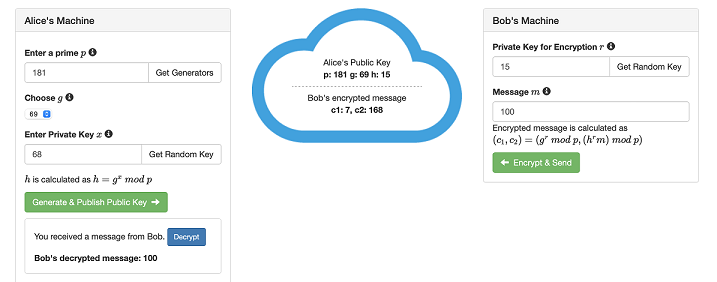
\includegraphics{externalExample.png}%
    \centering 
    \caption{Values generated by external site}%  
\end{figure}%
As it can be seen, the result of our program is the same as the result of the external website.
\newpage
\subsection{Test for large prime}
\begin{figure}[h]%
    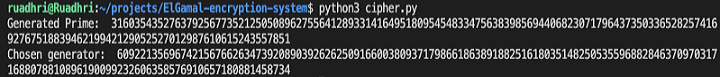
\includegraphics{largePrime.PNG}%
    \centering 
    \caption{Values generated by the script}%  
\end{figure}%
\begin{figure}[h]%
    \centering
    \subfloat{{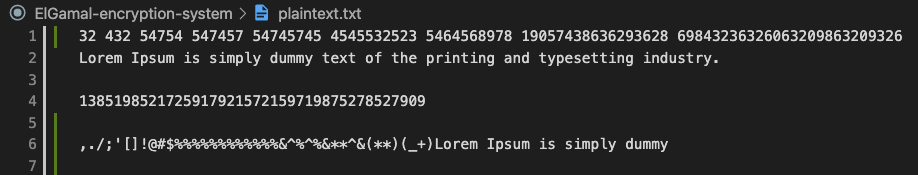
\includegraphics[width=15cm]{plaintextForLargePrime.png} }}%
    \qquad
    \subfloat{{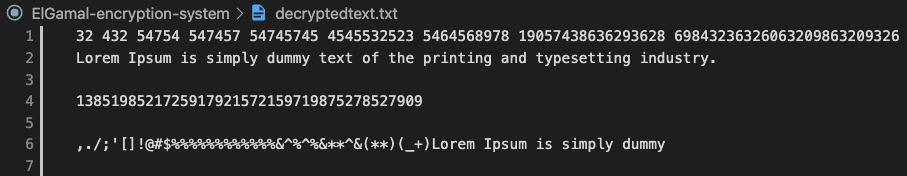
\includegraphics[width=15cm]{decryptedForLargePrime.png} }}%
    \caption{Plain text vs decrypted text}%
\end{figure}
\end{document}